
%------------------------------------------------

\newpage

\section{Random number correlation}
\label{exer:random_number_corr}

\subsection{Random number correlation in Metropolis–Hastings algorithm}

\begin{enumerate}
	\item Generate $10^{5} + 1$ random numbers distributed as a Gaussian with $\mu = 3$ and $\sigma = 2$.
	\item Plot the distributions of $x_{i}$ and of $\delta x_{i} = (x_{i} - x_{i - 1})$.
	\item Repeat by generating the numbers $x_{i}$ with the Metropolis-Hastings algorithm until $10^{5} + 1$ points are accepted.
	\item As a proposal function, use a Gaussian with $\mu_{p} = x_{i}$ and $\sigma = 0.3$.
	\item How do the distributions look like?
	\item Can you explain the standard deviation of the $\delta x_{i}$ distribution in the two cases?
\end{enumerate}

(Figure~\ref{fig:random_number_corr})

\begin{figure}
	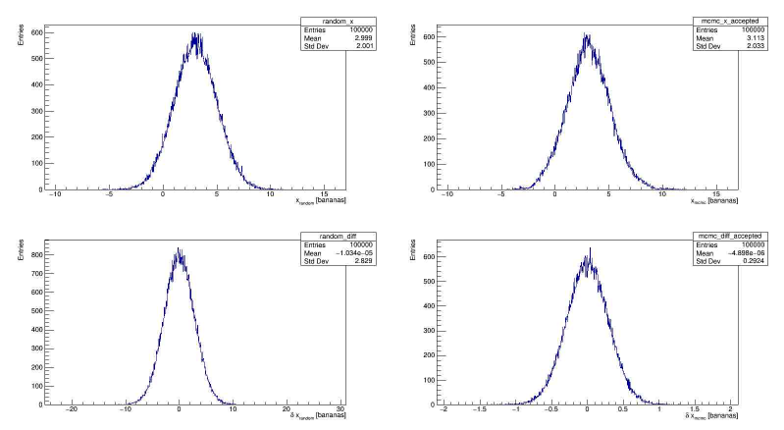
\includegraphics{exercise/random_number_corr.png}
	\caption[Random number correlation in Metropolis–Hastings algorithm.][6pt]{Random number correlation in Metropolis–Hastings algorithm.}
	\label{fig:random_number_corr}
\end{figure}

($\hookleftarrow$ \ref{subsec:prop_of_metropolis})
